\subsection{Presentaci\'on del problema y explicaci\'on del m\'etodo de discretizaci\'on}
Para averiguar la posici\'on de la isoterma debemos determinar la temperatura en cada punto de la pared. Al sernos imposible resolver el problema computacionalmente decidimos discretizar el problema, por lo que vamos a buscar las temperaturas cada una cierta distancia (la cual variaremos para experimentar los cambios en los resultados). Identificaremos as\'i un punto de la pared por su distancia al centro del horno (r) y su \'angulo ($\theta$) con respecto a un eje fijo.

Para determinar la temperatura en un punto contamos con la siguiente ecuaci\'on:

\begin{equation}\label{calor}
\frac{\partial^2T(r,\theta)}{\partial r^2}+\frac{1}{r}\frac{\partial T(r,\theta)}{\partial r}+\frac{1}{r^2}\frac{\partial^2T(r,\theta)}{\partial \theta^2} = 0 
\end{equation}

Siendo T($r$,$\theta$) la funci\'on que nos da como resultado la temperatura en un punto de radio r y \'angulo $\theta$.

Discretizamos tomando r$_i$ = r$_0$ \textless r$_1$ \textless ... \textless r$_n$ = r$_e$ (con r$_i$=radio interno y r$_e$=radio externo) y 0 = $\theta _0$ \textless $\theta _1$ \textless ... \textless $\theta _m$ = 2$\pi$, tomando así n+1 radios y m \'angulos. Por ende tomamos un t que cumple: t$_{i,j}$ = T(r$_i$,$\theta _j$) (temperatura en el punto con distancia r$_i$ al centro y \'angulo $\theta _j$).

Por ende tomamos la ecuaci\'on \ref{calor} y discretizando tenemos:

\begin{equation}
\label{EcuacionLaPlace}
\frac{t_{i-1,j}-2t_{i,j}+t_{i+1,j}}{(\Delta r)^2}+\frac{1}{r}\frac{t_{i+1,j}-t_{i,j}}{\Delta r}+\frac{1}{r^2}\frac{t_{i,j-1}-2t_{i,j}+t_{i,j+1}}{(\Delta \theta)^2}
\end{equation}

Con $\Delta r$ = r$_i$ - r$_{i-1}$ para i=1..n y $\Delta \theta$ = $\theta _j$ - $\theta _{j-1}$ para j=1..m.

Como vemos en la ecuaci\'on \ref{EcuacionLaPlace} la temperatura en un punto i,j (t$_{i,j}$) depende de las temperatura de los 4 puntos mas cercanos (t$_{i-1,j}$, t$_{i+1,j}$, t$_{i,j-1}$, t$_{i,j+1}$).

Si planteamos un sistema de ecuaciones con 1 ecuaci\'on para cada i,j de la discretizaci\'on obtenemos un sistema de n*m ecuaciones donde cada una depende de 5 temperaturas. Al mismo tiempo sabemos de antemano los valores de los puntos externos e internos, teniendo en cuenta que tomamos como par\'ametros conocidos la temperatura en el borde externo de la pared (T$_e$) y la temperatura en el borde interno de la pared (T$_i$).

\begin{figure}[ht]
\begin{center}
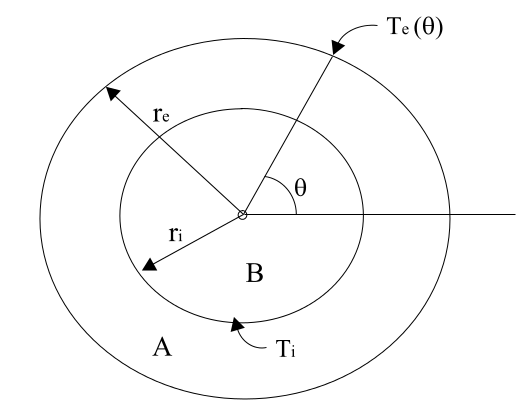
\includegraphics[width=0.4\columnwidth]{../tp1-package/docs/Horno.png}
\end{center}
\end{figure}

De esta forma, podemos plantear una matriz que cumple con la propiedad de ser banda, y con la cual además, es posible realizar Eliminación Gaussiana sin pivoteo (esta propiedad está demostrada más adelante).

\subsection{Armado de la Matriz Banda}
\label{subsec:DemBanda}

\par Para generar la matriz es necesario realizar una transformaci\'on del espacio polar en el que existen los puntos del horno (cuyas posiciones est\'an dadas por \'angulo y radio) a un vector de dimensi\'on (m + 1) * n (este valor corresponde con la cantidad de puntos en la discretizacio\'n). 
\par La transformaci\'on utilizada es bastante simple: 
\begin{equation}
f(j, k)\ =\ j * n + k
\label{eqTransf}
\end{equation}
donde f es la transformaci\'on, j representa que el elemento es el j-\'esimo en la componente del radio, k el equivalente para el \'angulo, y n es la cantidad de puntos de la discretizaci\'on con igual radio (la cantidad de puntos en cada c\'irculo conc\'entrico del horno).
\par De acuerdo a la ecuaci\'on \ref{EcuacionLaPlace}, para cada punto $p_{j, k}$ (cuya ecuaci\'on se encuentra representada en la fila $f(j, k)$) que no pertenece ni al radio externo ni al interno, los \'unicos coeficientes no-nulos en su fila corresponden a los puntos $p_{j-1, k}$, $p_{j+1, k}$, $p_{j, k}$, $p_{j, k-1}$, $p_{j, k+1}$; siendo los sub\'indices la posici\'on de cada punto en la discretizaci\'on. 
Utilizando la ecuaci\'on \ref{eqTransf}, estas posiciones corresponden a las siguientes columnas, respectivamente: $(j-1) * n + k$, $(j+1) * n + k$, $j * n + k$, $j * n + k - 1$, $j * n + k + 1$. 
\par k, como se ha dicho, representa al k-\'esimo elemento con radio j; ya que hay n elementos con igual radio, $0\leq k\leq n$. Por ende, para $j > 0$ ($j = 0$ corresponde al radio interno, por lo que este caso no nos concerniene en este momento), $j * n >= k$. 
Por lo tanto, la posici\'on de los valores de la diagonal en cada fila es $j*n+k$, y los valores no-nulos m\'as alejados corresponden a $(j-1) * n + k$ y $(j+1) * n + k$, que entonces equidistan $n$ de la diagonal. 
\par Es decir, se cumple la propiedad de banda para todas las filas de la matriz que no pertenecen al radio interno o externo, y el ancho de la banda es $n+1$. 
Sin embargo, queda justificar que la propiedad de banda se cumple para todas las dem\'as filas. 
Esto es simple de probar, ya que los valores de temperatura de cada uno de los puntos de estos radios son conocidos, y su ecuaci\'on est\'a simplemente dada por $t_{j, k}\ =\ b_{j, k}$; donde el primer t\'ermino representa la temperatura del punto y el segundo el valor del t\'ermino independiente determinado por la entrada.
Por lo tanto, el \'unico coeficiente no-nulo de las filas de los radios externo e interno son los de la diagonal, cuyo valor es 1.
Ya que todos los otros valores son nulos, en particular lo son los que distan m\'as que $n$ de la diagonal, y por ende la matriz es banda. Adicionalmente, hay $n$ puntos en el radio interno, por lo que la altura de la banda tambi\'en es $n+1$.
\par El algoritmo que crea la matriz en cuestión se encuentra en el apéndice B con comentarios incluidos, junto con el algoritmo correspondiente al método de Eliminación Gaussiana con aprovechamiento de matriz banda.

%\begin{figure}[ht]
%\begin{center}
%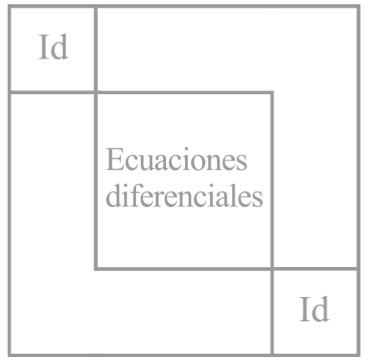
\includegraphics[width=0.4\columnwidth]{imagenes/banda.png}
%\caption{Armado de la Matriz Banda}
%\end{center}
%\end{figure}


\subsection{Demostración: Eliminación Gaussiana sin pivoteo}

\textbf{Proposici\'on}
\hfill{}
Sea $A \in \mathbb{R}^{n \times n}$ la matriz obtenida para el sistema. Es posible aplicar Eliminaci\'on Gaussiana sin pivoteo.

\subsubsection{Lema}

\par Sea $A \in \mathbb{R}^{n \times n}$ la matriz obtenida para el sistema, banda con ancho y alto $n+1$ (como se demostr\'o previamente). 
La \'ultima diagonal superior que pertenece a la banda, tiene (para los valores correspondientes a los radios no-externo y no-internos) coeficientes positivos.
Adicionalmente, al aplicar Eliminaci\'on Gaussiana estos coeficientes nunca se modifican. \newline

\textbf{}
\textbf{}
\textbf{Demostraci\'on del Lema}

\par El hecho que los coeficientes iniciales de la \'ultima diagonal (superior) de la banda sean positivos se desprende de las ecuaciones de cada punto, y ya se explic\'o previamente.
El hecho de que \'estos no se modifiquen al aplicar Gauss se debe a la estructura banda de la matriz:
\begin{equation}
A_{i, j} = 0\ si\ j < i - (n+1) \vee j > i + (n +1)
\end{equation}
\par Entonces, si $j = i + (n+1)$ (como es el caso de la \'ultima diagonal superior de la banda), para una fila $i$, para todas las filas anteriores $k < i$, $j > k + (n+1)$, por lo que $A_{k, j} = 0$.
Al ser $0$, al aplicar Gauss no se alterar\'a el valor del coeficiente.

\subsubsection{Demostraci\'on de la proposici\'on}

\par Ya detallamos que la ecuaci\'on de cada punto indica que en cada fila, la diagonal m\'as la suma de todos los otros coeficientes (no nulos, y luego de todos) es 0. Es decir:
\begin{equation}
A_{i, i} = - (\sum_{j\neq i} A_{i, j})
\end{equation}
\par Por ende, 
\begin{equation}
    \abs{A_{i, i}} = \abs{(\sum_{j\neq i} A_{i, j})} = (\sum_{j\neq i} \abs{A_{i, j}}) \geq (\sum_{j\neq i} \abs{A_{i, j}})
\end{equation}
\par El m\'odulo de la suma es igual a la suma de los m\'odulos ya que todos los coeficientes son no-negativos.
De acuerdo a la ecuaci\'on anterior, la matriz es diagonal dominante (aunque no estrictamente).
\par Demostraremos por inducci\'on que dadas estas propiedades, se puede realizar Eliminaci\'on Gaussiana sin pivoteo.\newline
\newline
\textbf{Caso Base}


\par El caso base consiste en la matriz creada inicialmente, que como ya se demostr\'o, es diagonal dominante, y los valores de su diagonal son no-nulos (para los radios interno y externo valen 1, y
para los otros ya se demostr\'o que son no-nulos).\newline
\newline
\textbf{}
\textbf{Paso Inductivo}


\par Si A tras realizar $k$ iteraciones de Gauss sin pivotaje es diagonal dominante, con $A_{k, k}$ (es decir, el $k$-\'esimo valor de la diagonal) no-nulo, entonces A tras realizar $k+1$ iteraciones de Gauss sin pivotaje es diagonal dominante, con $A_{k+1, k+1}$ no-nulo.
\par Demostraremos primero que A tras realizar $k+1$ iteraciones es diagonal dominante.
Restamos cada fila inferior a la $k$ por el coeficiente correcto:
\begin{equation}
A_j - (A_{j, k} / A_{k, k}) * A_k
\end{equation}
\par Sabemos que es posible hacer esto ya que por Hip\'otesis Inductiva $A_{k, k} \neq 0$.
Sea
\begin{equation}
A_{i, j}^{(2)} = A_{i, j} - (A_{i, k} / A_{k, k}) * A_{k, j}
\end{equation}
\par Quiero ver que:
\begin{equation}
\sum_{j\neq\ i}\abs{A_{i, j}^{(2)}}\leq\ \abs{A_{i, i}^{(2)}}
\end{equation}
\par Veamos que esto sucede:
\begin{equation}
\sum_{j\neq\ i}\abs{A_{i, j} - (A_{i, k} / A_{k, k}) * A_{k, j}}
\end{equation}
\par Por Desigualdad Triangular:
\begin{equation}
    ...\ \leq\ \sum_{j\neq\ i}\abs{A_{i,j}} + \sum_{j\neq\ i}\abs{(A_{i, k} / A_{k, k})}
\end{equation}
\par Por Hip\'otesis Inductiva:
\begin{equation}
    ...\ \leq\ \abs{A_{i, i}} - \abs{A_{i, k}} + (\abs{A_{i, k}}/ \abs{A_{k, k}})*(\sum_{j\neq i}\abs{A_{k, j}})
\end{equation}
\begin{equation}
    ...\ \leq\ \abs{A_{i, i}} - \abs{A_{i, k}} + (\abs{A_{i, k}}/ \abs{A_{k, k}})*(\abs{A_{k, k}}-\abs{A_{k, i}})
\end{equation}
\begin{equation}
    ...\ \leq\ \abs{A_{i, i}} - \abs{A_{i, k}} * \abs{A_{k, i}} / \abs{A_{k, k}}
\end{equation}
\begin{equation}
    ...\ \leq\ \abs{A_{i, i}} 
\end{equation}
\par Finalmente, llegamos a que cada fila donde se rest\'o por Gauss sin pivotaje mantiene su propiedad de diagonalidad dominante (no estricta).
\par Probamos la primera de las dos propiedades que quer\'iamos demostrar: a\'un queda justificar que $A_{k+1, k+1}$ es no-nulo luego de la $k+1$-\'esima iteraci\'on.
+Afortunadamente, esta demostraci\'on es m\'as simple. Utilizando la misma notaci\'on que en la demostraci\'on de la propiedad anterior:
\begin{equation}
A_{k+1, k+1}^{(2)} = A_{k+1, k+1} - (A_{k+1, k} / A_{k, k}) * A_{k, k+1}
\end{equation}
\par En particular, queremos ver que $A_{k+1, k+1}^{(2)}\neq\ 0$:
\begin{equation}
A_{k+1, k+1}^{(2)} \neq 0\ \iff A_{k+1, k+1} - (A_{k+1, k} / A_{k, k}) * A_{k, k+1} \neq 0
\end{equation}
\par De esto se desprende:
\begin{equation}
A_{k+1, k+1} \neq (A_{k+1, k} / A_{k, k}) * A_{k, k+1}
\end{equation}
\par Aplicando m\'odulo de ambos lados de la inecuaci\'on:
\begin{equation}
    \abs{A_{k+1, k+1}} \neq \abs{(A_{k+1, k}} / \abs{A_{k, k})} * \abs{A_{k, k+1}}
\end{equation}
\par Por Hip\'otesis Inductiva, sabemos que 
\begin{equation}
    \abs{A_{k+1, k+1}} \geq \abs{(A_{k+1, k}} 
\end{equation}
\begin{equation}
    \abs{A_{k, k})} \geq \abs{A_{k, k+1}}
\end{equation}
\par La \'unica forma en que se podr\'ia anular $A_{k+1, k+1}$ es si ambos valores de la diagonal son exactamente iguales a $A_{k, k+1}$ y $A_{k+1, k}$, respectivamente.
\par Sin embargo, esto no puede suceder, debido al Lema que demostramos al comienzo de esta prueba: los valores de la \'ultima diagonal de la banda (que debido a la forma de la matriz, nunca ser\'an
$A_{k, k+1}$ o $A_{k+1, k}$) son no-nulos (y en particular positivos, pero con no-nulos alcanza). Si pasara que $\abs{A_{k, k})} = \abs{A_{k, k+1}}$ (o lo mismo para el otro par de valores), entonces:
\begin{equation}
    \abs{A_{k, k})} < \abs{A_{k, k+1}} + \abs{A_{k, k+(n+1)}}
Add a comment to this line
\end{equation}
\par Esto es absurdo, ya que por Hip\'otesis Inductiva, A es diagonal dominante.
\par $QED$.



\subsection{Planteo de Algoritmos}
\par Para el armado de los algoritmos partimos de una división de los subproblemas a resolver:
\begin{itemize}
\item Crear la matriz en base al archivo de entrada, calculando los coeficientes a partir de las ecuaciones y ordenándolos de tal forma que quede banda, como se explicó anteriorimente.
\item Resolver la matriz con el método de Gauss.
\item Calcular la L y la U.
\item Resolver en base a una L y una U.
\item Calcular la isoterma, con dos métodos diferentes: el primero, calculando el radio más cercano al valor buscado por cada ángulo; y el segundo, aproximando un valor entre los dos radios más cercanos al valor buscado.
\item Determinar si es peligroso, de dos maneras diferentes: la primera viendo si algún punto de la isoterma sobrepasa un radio predeterminado cercano al radio externo, y la segunda calculando el porcentaje de puntos que sobrepasan dicho límite. 
\end{itemize}

\par Algunos algoritmos los planteamos basándonos en sus versiones conocidas (y vistas en clase): método de Gauss y calculo de la L y la U. Luego los modificamos de acuerdo a algunos temas de optimización y detalles para las entradas particulares del problema a resolver.
\par Pasamos por una etapa de prueba de los algoritmos, tanto individualmente como en conjunto, donde tuvimos que dedicarnos a algunos errores que surgieron en cuanto a índices y casos borde.
\par Una vez terminados, optimizamos el algoritmo de Eliminación Gaussiana para matrices Banda. Como se puede ver en el apéndice B, el código aprovecha la propiedad de los 0s fuera de la sección diagonal para realizar menos iteraciones.
\par Teníamos planteado implementar las estructuras para aprovechar la propiedad de banda y reducir la complejidad espacial del algoritmo, pero por cuestiones de tiempo, decidimos enfocarnos en la experimentación y discusión.
\par Finalmente nos dedicamos a aproximar la isoterma de mejor manera y pasamos a experimentar. 

\subsection{Planteo de Mediciones Experimentales}

\par Dividiremos los experimentos realizados en tres secciones, dependiendo el aspecto del algoritmo que se quiere medir y comparar.
\begin{itemize}


\item Complejidad Temporal: experimentos que apuntan a comparar el costo en tiempo de ejecución de los algoritmos, dependiendo del nivel de la granularidad (Experimento 1), del método escogido con temperaturas dinámicas, Gauss o LU (Experimento 2), y la comparación con el método que aprovecha el hecho de que la matriz sea banda (Experimento 3).
\item Isoterma: experimentos que apuntan a comparar cómo varía la isoterma devuelta por el algoritmo modificando la granularidad de los radios (Experimento 4), granularidad de los ángulos (Experimento 5) y granularidad de radios y ángulos a la vez (Experimento 6). Además, se comparan dos métodos para calcular la isoterma: el primero, redondeando el resultado al radio más cercano correspondiente al valor buscado en cada ángulo; y el segundo, que calcula un promedio entre los radios más cercanos al valor buscado (Experimento 7). Un último experimento (Experimento 8) busca corroborar si vale la pena aumentar la granularidad para obtener resultados más precisos, en contraposición con un método menos costoso pero de menor precisión.
\item Peligrosidad: experimentos que buscan comparar los dos métodos implementados para calcular la peligrosidad del horno según la isoterma (Experimento 9). El primer método, más brusco, busca solamente si un punto de la isoterma haya traspado el valor de la isoterma 500, mientras que el segundo, realiza un cálculo de porcentaje para calcular si la cantidad de puntos del horno en peligro supera un umbral predeterminado.
\end{itemize}

